%! alt Triangle ABC with K on BC beyond C. Through K, KP is parallel to AB with BP = BK, and KQ is parallel to AC with CQ = CK. The circle through K, P and Q meets AK again at T. The auxiliary point D, with triangle CTD similar to triangle CQA, is joined to A, B, C and T, and the dashed segments AP, AQ, BT, CT, PT and QT show the two similar pairs used in the proof. Adapted from Beyond the Incenter, Problem 86.
%! after_paragraph 1
%! scale 4/7
% The shared preamble of every Cevian figure. pipeline/figures turns these colours into theme-aware paint,
% and refuses any other colour, so draw only with them:
%   figink (lines and labels), figaux (construction lines), figaccent (the object the argument turns on),
%   figtint and figaccenttint (light fills).
\documentclass[border=1.5pt]{standalone}
\usepackage{tkz-euclide}
\definecolor{figink}{RGB}{0,0,0}
\definecolor{figaux}{RGB}{85,85,85}
\definecolor{figaccent}{RGB}{192,57,43}
\definecolor{figtint}{RGB}{221,221,221}
\definecolor{figaccenttint}{RGB}{245,213,208}
% tkz-euclide's defaults draw circles, compasses and marks in 50% grey and fill points with a tint.
\makeatletter
\def\tkz@otherlinecolor{figink}
\def\tkz@euc@circlecolor{figink}
\def\tkz@euc@compasscolor{figink}
\def\tkz@euc@mkcolor{figink}
\def\tkz@mk@fill{figink}
\def\tkz@euc@pointfillcolor{figink}
\makeatother
\tkzSetUpLine[color=figink,line width=.7pt]
\tkzSetUpArc[color=figink,line width=.7pt]
\tkzSetUpCompass[color=figink,line width=.5pt]
\tkzSetUpPoint[color=figink,fill=figink,size=3.1pt]
\tikzset{
  every picture/.style={line cap=round,line join=round,color=figink},
  circle style/.append style={color=figink,line width=.7pt},
  aux/.style={color=figaux,line width=.45pt,dash pattern=on 2.6pt off 2pt},
  key/.style={color=figaccent,line width=1pt},
  mk/.style={color=figink,line width=.5pt},
  lbl/.style={color=figink,inner sep=2.2pt},
  len/.style={color=figink,inner sep=1.5pt,font=\small},
}

\begin{document}
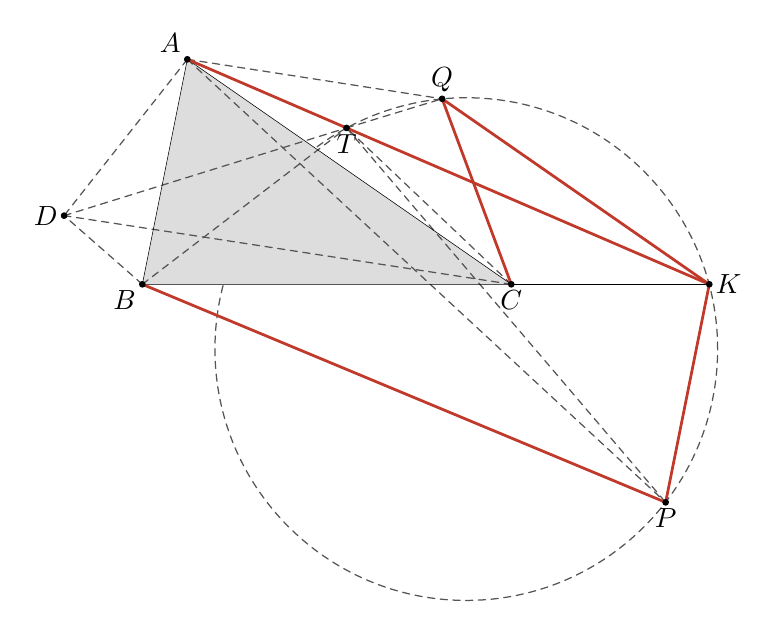
\begin{tikzpicture}
%! let ax = -2
%! let ay = 5
%! let cx = 26/5
%! let kx = 48/5
\tkzDefPoint(-1.1428571,2.8571429){A} %! A = (ax, ay)
\tkzDefPoint(-1.7142857,0.0){B} %! B = (-3, 0)
\tkzDefPoint(2.9714286,0.0){C} %! C = (cx, 0)
\tkzDefPoint(5.4857143,0.0){K} %! K = (kx, 0)
\tkzDefPoint(4.9318681,-2.7692308){P} %! P = lerp(K, foot(B, K, shift(K, 1, 5)), 2)
\tkzDefPoint(2.0931955,2.3559158){Q} %! Q = lerp(K, foot(C, K, shift(K, cx - ax, -ay)), 2)
\tkzDefPoint(2.4000000,-0.82285714){O} %! O = circumcentre(K, P, Q)
\tkzDefPoint(0.87944705,1.9854600){T} %! T = lerp(K, foot(O, A, K), 2)
%! let ux = ax - cx
%! let uy = ay
%! let vx = x(T) - cx
%! let vy = y(T)
%! let wx = x(Q) - cx
%! let wy = y(Q)
%! let nx = ux*vx - uy*vy
%! let ny = ux*vy + uy*vx
%! let ww = wx**2 + wy**2
\tkzDefPoint(-2.7080185,0.87168284){D} %! D = (cx + (nx*wx + ny*wy)/ww, (ny*wx - nx*wy)/ww)
%! fact parallel(K, P, A, B)
%! fact parallel(K, Q, A, C)
%! fact equal(dist(B, P), dist(B, K))
%! fact equal(dist(C, Q), dist(C, K))
%! fact collinear(T, A, K)
%! fact concyclic(K, P, Q, T)
%! fact equal(angle(T, C, D), angle(Q, C, A))
%! fact equal(dist(C, D)*dist(C, Q), dist(C, A)*dist(C, T))
%! fact equal(angle(B, A, D), angle(B, P, T))
%! fact equal(dist(A, P)*dist(B, T)*dist(C, Q), dist(A, Q)*dist(C, T)*dist(B, P))
\tkzDrawCircle[aux](O,K)
\tkzFillPolygon[color=figtint](A,B,C)
\tkzDrawSegments[aux](A,D B,D C,D D,T B,T C,T A,Q T,Q A,P T,P)
\tkzDrawPolygon(A,B,C)
\tkzDrawSegment(C,K)
\tkzDrawSegments[key](K,P K,Q A,K B,P C,Q)
\tkzDrawPoints(A,B,C,K,P,Q,T,D)
\tkzLabelPoint[above left,lbl](A){$A$}
\tkzLabelPoint[below left,lbl](B){$B$}
\tkzLabelPoint[below,lbl](C){$C$}
\tkzLabelPoint[right,lbl](K){$K$}
\tkzLabelPoint[below,lbl](P){$P$}
\tkzLabelPoint[above,lbl](Q){$Q$}
\tkzLabelPoint[below,lbl](T){$T$}
\tkzLabelPoint[left,lbl](D){$D$}
\end{tikzpicture}
\end{document}
